\documentclass[12pt,a4paper]{article}
\usepackage{tabularx}
\usepackage{booktabs}
\usepackage{longtable}
\usepackage{ltxtable}
\usepackage[latin1]{inputenc}
\usepackage{amssymb}
\usepackage[]{graphicx,rotating}
\usepackage[T1]{fontenc}
\usepackage{parskip}
\usepackage{listings}
\usepackage{natbib}
\usepackage[official]{eurosym}
\usepackage{mathrsfs}
\usepackage{amsmath}
\usepackage{verbatim}
\usepackage[usenames,dvipsnames]{color}     %for R colors and formatting

\usepackage[left=3cm, right=2.5cm, top=2.5cm]{geometry}

\pagestyle{empty}
\parindent 0cm
\renewcommand{\baselinestretch}{1}
\newcommand{\bs}{\boldsymbol}
\renewcommand{\familydefault}{cmss}
\pdfminorversion=7
\bibliographystyle{agsm}

\lstset{ %for R colors and formatting
  language=R,                     % the language of the code
  basicstyle=\scriptsize\ttfamily, % the size of the fonts that are used for the code
  numbers=left,                   % where to put the line-numbers
  numberstyle=\scriptsize\color{Blue},  % the style that is used for the line-numbers
  stepnumber=1,                   % the step between two line-numbers. If it is 1, each line
                                  % will be numbered
  numbersep=5pt,                  % how far the line-numbers are from the code
  backgroundcolor=\color{white},  % choose the background color. You must add \usepackage{color}
  showspaces=false,               % show spaces adding particular underscores
  showstringspaces=false,         % underline spaces within strings
  showtabs=false,                 % show tabs within strings adding particular underscores
  frame=single,                   % adds a frame around the code
  rulecolor=\color{black},        % if not set, the frame-color may be changed on line-breaks within not-black text (e.g. commens (green here))
  tabsize=2,                      % sets default tabsize to 2 spaces
  captionpos=b,                   % sets the caption-position to bottom
  breaklines=true,                % sets automatic line breaking
  breakatwhitespace=false,        % sets if automatic breaks should only happen at whitespace
  keywordstyle=\color{RoyalBlue},      % keyword style
  commentstyle=\color{YellowGreen},   % comment style
  stringstyle=\color{ForestGreen}      % string literal style
} 

\begin{document}

\begin{center}
% \vspace*{1cm}
 
\includegraphics[width=0.35\textwidth]{GU-Logo-blau-CMYK.eps} \vspace{2cm}
  
  {\Large{\bf Predicting Cross-Sell with Artificial Neural Networks}} \newline
  {\Large{An Empirical Study of ING's Customer Data}} \vspace{0.5cm}

  Seminar Thesis \\\vspace{2cm}
  submitted to \\\vspace{0.5cm}
  \textbf{Hon.-Prof. Dr. Martin Schmidberger} \\
  \textbf{Gabriela Alves Werb} \\\vspace{0.5cm}
  Goethe University Frankfurt am Main \\
  School of Business and Economics \\
  Chair for E-Commerce \vspace{2cm}
  
  by \\\vspace{0.5cm}
  \textbf{Lukas J\"urgensmeier} \\
  (Mat.-Nr.: 6904281) \\
  
  \medskip
  \medskip
  in partial fulfillment of the requirements \\
  for the degree of \\\vspace{0.5cm}
  \textbf{Master of Science in Business Administration} \\\vspace{0.5cm}
  July 31, 2019
  
\end{center}


\pagebreak
\pagestyle{plain}
\pagenumbering{Roman}
\tableofcontents
\listoffigures
\listoftables
\newpage
\setcounter{page}{2}
\pagenumbering{arabic}
\setlength{\baselineskip}{1.5\baselineskip}
\pagestyle{plain}


\section{Introduction}
The introduction should directly lead to the main topic of the paper. It
should not be a historical essay or a deep reaching explanation of
the topic, but it should explain concisely what the main questions
of the topic are, why they are interesting, and which methods or
data will be used. A further goal of the introduction is to define the
structure for the paper. This can be achieved by describing
the goals, the methods and the main results of the paper.
Methods and results do not have to be
discussed in detail - this is left to the main part of the paper -
 but they should be summed up in a short way.
 The introduction of a paper is often finished by a short ``roadmap''.
 This is not necessary, if the aspects mentioned above have been
 laid out in a satisfactory way before. \citep{hastieElementsStatisticalLearning2017} This is a reference test from the new .tex file \ref{fig:average2}

\section{Introduction from different file}

The introduction should directly lead to the main topic of the paper. It
should not be a historical essay or a deep reaching explanation of
the topic, but it should explain concisely what the main questions
of the topic are, why they are interesting, and which methods or
data will be used. A further goal of the introduction is to define the
structure for the paper. This can be achieved by describing

\begin{figure}[!h]
\begin{center}\caption{Mean Bond-Yield-curve (example for a figure)\label{fig:average2}}

\includegraphics[width=100mm]{GU-Logo-blau-CMYK.eps}\\
\tiny Mean Nelson-Siegel Bond-Yield-curve compared to the realized
Bond-Yields.
\end{center}
\end{figure}

\begin{figure}[!h]
\begin{center}\caption{Example from the CSCC lecture\label{fig:CSCC_plot}}
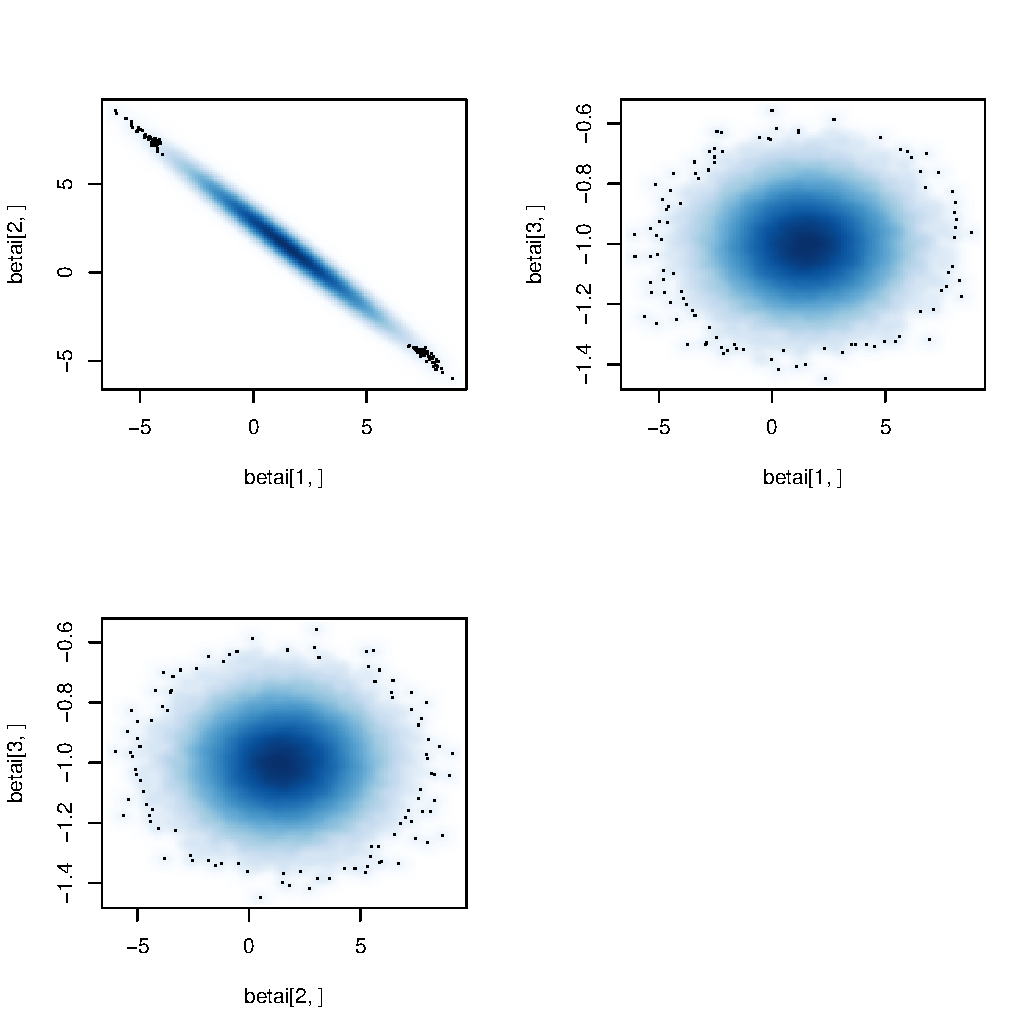
\includegraphics[width=\textwidth]{figures/CSCC_plots.pdf}\\
\tiny I have no clue what this figure is all about.
\end{center}
\end{figure}


the goals, the methods and the main results of the paper.
Methods and results do not have to be
discussed in detail - this is left to the main part of the paper -
 but they should be summed up in a short way.
 The introduction of a paper is often finished by a short ``roadmap''.
 This is not necessary, if the aspects mentioned above have been
 laid out in a satisfactory way before. \citep{hastieElementsStatisticalLearning2017}

\begin{lstlisting}[language=R,caption={Tensorflow Model}, label=lst:tensorflow]
# This script follows this blog post
# https://blogs.rstudio.com/tensorflow/posts/2018-01-11-keras-customer-churn/

# clear workspace
rm(list = ls())

#install packages
#pkgs <- c("keras", "lime", "tidyquant", "rsample", "recipes", "yardstick", "corrr")
#install.packages(pkgs)

# Load libraries
library(keras)
library(lime)
library(tidyquant)
library(rsample)
library(recipes)
library(yardstick)
library(corrr)


# Install Keras if you have not installed before
install_keras(method = "conda")

# read and check data
xsell_data_raw <- read.csv("xsell.csv")
glimpse(xsell_data_raw)

# create new variable tenure
xsell_data_raw$tenure <- xsell_data_raw$age - xsell_data_raw$entry_age

# prune data set
# Remove unnecessary data
xsell_data_tbl <- xsell_data_raw %>%
  select(-X) %>% #removes ID
  drop_na() #%>% # removes all NA's. Bad Solution! Improve! Removes 70% of observations
 # select(xsell, everything())
glimpse(xsell_data_tbl)

# Split test/training sets
set.seed(123)
train_test_split <- initial_split(xsell_data_tbl, prop = 0.8)
train_test_split

# Retrieve train and test sets
train_tbl <- training(train_test_split)
test_tbl  <- testing(train_test_split)

# skipped all feature transformations here
# insert if necessary

# # alternative way for dummy coding all non-numeric variables
# non_numeric_var_names <- xsell_data_tbl %>%
#   select_if(negate(is.numeric)) %>%
#   names
# 
# xsell_data_tbl <- dummy_cols(xsell_data_tbl, non_numeric_var_names)
# 
# # remove non-numeric variables
# xsell_data_tbl <- xsell_data_tbl %>%
#   select(-non_numeric_var_names)
# glimpse(xsell_data_tbl)

# Create recipe
rec_obj <- recipe(xsell ~ ., data = train_tbl) %>%
  #step_discretize(tenure, options = list(cuts = 6)) %>%
  #step_log(TotalCharges) %>%
  step_dummy(all_nominal(), -all_outcomes()) %>%
  step_center(all_predictors(), -all_outcomes()) %>%
  step_scale(all_predictors(), -all_outcomes()) %>%
  prep(data = train_tbl)

# Apply recipe to predictors (all vars excluding xsell)
x_train_tbl <- bake(rec_obj, new_data = train_tbl) %>% select(-xsell)
x_test_tbl  <- bake(rec_obj, new_data = test_tbl) %>% select(-xsell)
glimpse(x_train_tbl)

# define response variables for training and testing sets
y_train_vec <- pull(train_tbl, xsell)
y_test_vec  <- pull(test_tbl, xsell)


# Building our Artificial Neural Network
model_keras <- keras_model_sequential()

model_keras %>% 
  
  # First hidden layer
  layer_dense(
    units              = 16, 
    kernel_initializer = "uniform", 
    activation         = "relu", 
    input_shape        = ncol(x_train_tbl)) %>% 
  
  # Dropout to prevent overfitting
  layer_dropout(rate = 0.1) %>%
  
  # Second hidden layer
  layer_dense(
    units              = 16, 
    kernel_initializer = "uniform", 
    activation         = "relu") %>% 
  
  # Dropout to prevent overfitting
  layer_dropout(rate = 0.1) %>%
  
  # Output layer
  layer_dense(
    units              = 1, 
    kernel_initializer = "uniform", 
    activation         = "sigmoid") %>% 
  
  # Compile ANN
  compile(
    optimizer = 'adam',
    loss      = 'binary_crossentropy',
    metrics   = c('accuracy')
  )

keras_model

history <- fit(
  object           = model_keras, 
  x                = as.matrix(x_train_tbl), 
  y                = y_train_vec,
  batch_size       = 50, 
  epochs           = 35,
  validation_split = 0.30
)

# Print a summary of the training history
print(history)

# Plot the training/validation history of our Keras model
plot(history)

# Make predictions
# Predicted Class
yhat_keras_class_vec <- predict_classes(object = model_keras, x = as.matrix(x_test_tbl)) %>%
  as.vector()

# Predicted Class Probability
yhat_keras_prob_vec  <- predict_proba(object = model_keras, x = as.matrix(x_test_tbl)) %>%
  as.vector()

# Evaluate model
# Format test data and predictions for yardstick metrics
estimates_keras_tbl <- tibble(
  truth      = as.factor(y_test_vec), # %>% fct_recode(yes = "1", no = "0"),
  estimate   = as.factor(yhat_keras_class_vec), # %>% fct_recode(yes = "1", no = "0"),
  class_prob = yhat_keras_prob_vec
)

estimates_keras_tbl

# change default positive=0 to positive=1
options(yardstick.event_first = FALSE)

# Confusion Table
estimates_keras_tbl %>% conf_mat(truth, estimate)

# Accuracy
estimates_keras_tbl %>% metrics(truth, estimate)

# AUC
estimates_keras_tbl %>% roc_auc(truth, class_prob)

# Precision
tibble(
  precision = estimates_keras_tbl %>% precision(truth, estimate),
  recall    = estimates_keras_tbl %>% recall(truth, estimate)
)

# F1-Statistic
estimates_keras_tbl %>% f_meas(truth, estimate, beta = 1)


####################################################
#### Evaluate Feature Importance with LIME #########
####################################################

# Setup
class(model_keras)

#Setup lime::model_type() function for keras
model_type.keras.engine.sequential.Sequential <- function(x, ...) {
  return("classification")
  }


# Setup lime::predict_model() function for keras
predict_model.keras.engine.sequential.Sequential <- function(x, newdata, type, ...) {
  pred <- predict_proba(object = x, x = as.matrix(newdata))
  return(data.frame(Yes = pred, No = 1 - pred))
  }


# Test our predict_model() function
predict_model(x = model_keras, newdata = x_test_tbl, type = 'raw') %>%
  tibble::as_tibble()

# Run lime() on training set
explainer <- lime::lime(
  x              = x_train_tbl, 
  model          = model_keras, 
  bin_continuous = FALSE
)

# Run explain() on explainer
explanation <- lime::explain(
  x_test_tbl[1:10, ], 
  explainer    = explainer, 
  n_labels     = 1, 
  n_features   = 4,
  kernel_width = 0.5
)

# Plot feature importance
plot_features(explanation) +
  labs(title = "LIME Feature Importance Visualization",
       subtitle = "Hold Out (Test) Set, First 10 Cases Shown")

plot_explanations(explanation) +
  labs(title = "LIME Feature Importance Heatmap",
       subtitle = "Hold Out (Test) Set, First 10 Cases Shown")

# Feature correlations to xsell
corrr_analysis <- x_train_tbl %>%
  mutate(xsell = y_train_vec) %>%
  correlate() %>%
  focus(xsell) %>%
  rename(feature = rowname) %>%
  arrange(abs(xsell)) %>%
  mutate(feature = as_factor(feature)) 

corrr_analysis

# Correlation visualization
corrr_analysis %>%
  ggplot(aes(x = xsell, y = fct_reorder(feature, desc(xsell)))) +
  geom_point() +
  # Positive Correlations - Contribute to churn
  geom_segment(aes(xend = 0, yend = feature), 
               color = palette_light()[[2]], 
               data = corrr_analysis %>% filter(xsell > 0)) +
  geom_point(color = palette_light()[[2]], 
             data = corrr_analysis %>% filter(xsell > 0)) +
  # Negative Correlations - Prevent churn
  geom_segment(aes(xend = 0, yend = feature), 
               color = palette_light()[[1]], 
               data = corrr_analysis %>% filter(xsell < 0)) +
  geom_point(color = palette_light()[[1]], 
             data = corrr_analysis %>% filter(xsell < 0)) +
  # Vertical lines
  geom_vline(xintercept = 0, color = palette_light()[[5]], size = 1, linetype = 2) +
  geom_vline(xintercept = -0.25, color = palette_light()[[5]], size = 1, linetype = 2) +
  geom_vline(xintercept = 0.25, color = palette_light()[[5]], size = 1, linetype = 2) +
  # Aesthetics
  theme_tq() +
  labs(title = "Cross Sell Correlation Analysis",
       subtitle = paste("Positive Correlations (contribute to xsell),",
                        "Negative Correlations (prevent xsell)"),
       y = "Feature Importance")

\end{lstlisting}


\section{Main part}
\subsection{Literature overview and citation}
The literature overview may be kept short in a bachelor thesis. Bachelor theses
 whose main purpose is to present and discuss the contents
of published articles are exceptions. When referring to articles or
other literature, it is essential to mark these as references. This is best


\begin{equation}\label{eq:xsquared}
  f(x) = x^2\\
\end{equation}
\begin{equation}\label{eq:integral}
  F(x) = \int^a_b \frac{1}{3}x^3
\end{equation}

done in the text itself. When referring to papers, the author
and the year of publication should be given, e.g. ``Imbens
(2002) gives an overview for the GMM-estimator and its empirical
likelihood''. See for example in \eqref{eq:xsquared} for the squared one
and \eqref{eq:integral} for an example of a fancy integral.


If the paper was written by more than two authors, this fact
is usually abbreviated as, for example, ``Imbens et al. (2002)''.
If there was more than one publication in the same year, a small letter should be added to
the year such as ``Imbens (1997a)''. When referring to a whole
chapter, the chapter should be mentioned, e.g. ``Wooldridge (2002),
ch. 13''.

Direct citations must be enclosed in quotation marks. In
this case the year of publication should be added with the author's
name, e.g. ``Generalized method of moments (GMM) estimation has
become an important unifying framework for inference in econometrics
in the last 20 years (Imbens (2002), p. 493)''. The use of direct
citations should be kept to a minimum.

\subsection{Theory and methods}
When writing an empirical bachelor thesis, the theoretical part should be
limited to an amount necessary to understand the empirical part. It
is better to limit the theory to the special cases rather
than striving for a maximum of generality. Of course,
when writing a theoretical paper, or a paper on pure methods,
the theoretical part will receive more weight. However,
the presentation should always be structured so that it clearly
works out the main points, concentrating on the aspects
that are really central to the topic. Detailed proofs should be moved
to the appendix.


\subsection{Data}

When writing an empirical paper, it is necessary to give a
concise description of the data set that is being used. This description
should include information about the data set provider and
the variables used. A descriptive analysis of the data is useful, but it may also be
moved to the appendix.

\subsection{Empirical Analysis}

In the empirical section, the main results should be
explained first. If this is not possible, because intermediate steps
are required to understand the results, then only
intermediate results should be explained that are really essential
for this purpose.  Tables and figures should be used to present
the main results. In addition, the tables and figures have to be
discussed in the text. Each table and each figure must have
their own title and caption.

It is often useful to investigate the robustness of the results
with respect to different aspects. If the results were calculated under
the homoskedasticity assumption for example, one should discuss what
happens if the assumption is violated. More detailed empirical results
should be put into the appendix unless there are important reasons not to do
so.

\section{Conclusion}

The conclusion should contain a summary of the main results and its implications. One can
also mention directions for future research.

\clearpage
\appendix
\section{R Code}
\begin{lstlisting}[language=R,caption={Fibonacci Secquence}, label=lst:testcode]
fib <- function(n) {
  if (n < 2)
    n
  else
    fib(n - 1) + fib(n - 2)
}
fib(10)
\end{lstlisting}

\begin{verbatim}
  fib <- function(n) {
  if (n < 2)
    n
  else
    fib(n - 1) + fib(n - 2)
}
fib(10)
\end{verbatim}

See Test Code \ref{lst:testcode} for the code example.

\section{Formatting rules}

\begin{center}
\begin{itemize}
\item Letter size 11 to 12pt, line spacing 1 - 1.5 times letter size, margins left/right 2.5cm, bottom 3cm, top 2.5cm.
\item Pre-introduction page numbers should be roman, the ones of the main text arabic.
\item The table of contents shows chapters and sections.
\item The list of figures and tables list all the figures and tables in the paper.
\item Every figure and table should have a short title plus description and should be explained in the text.
\item The number of pages of the main text should be between 10-15 pages (appendix excluded).
\end{itemize}
\end{center}



\begin{figure}[!h]
\begin{center}\caption{Mean Bond-Yield-curve (example for a figure)\label{fig:average}}

\includegraphics[width=100mm]{GU-Logo-blau-CMYK.eps}\\
\tiny Mean Nelson-Siegel Bond-Yield-curve compared to the realized
Bond-Yields.
\end{center}
\end{figure}

\begin{table}[h]\small
\begin{center}\caption{Cointegration of Bond Yields (example for a table)\label{tab:Coint}}
\begin{tabular}{lcccc}
& & & & \\
\hline
& & & & \\
Rank at least & $\mathscr{L}_{trace}$ & $5\%$ crit. value & $\mathscr{L}_{max}$ & $5\%$ crit. value \\
$r_0=0$ & 299.71 & 76.07 & 108.08 & 34.40 \\
$r_0=1$ & 191.64 & 53.12 & 91.00 & 28.14 \\
$r_0=2$ & 100.64 & 34.91 & 65.14 & 22.00 \\
$r_0=3$ & 35.50 & 19.96 & 29.29 & 15.67 \\
$r_0=4$ & 6.21 & 9.24 & 6.21 & 9.24 \\
\hline
\multicolumn{5}{l}{\tiny The Akaike-Information-criterion suggests a maximal lag length of 14}\\
\end{tabular}
\end{center}
\end{table}


\clearpage
\bibliography{library}

\newpage
\thispagestyle{empty}
\section*{Statutory Declaration}\label{statutory-declaration}

I herewith declare that I have completed the present thesis independently, without making use of
other than the specified literature and aids. Sentences or parts of sentences quoted literally are
marked as quotations; identification of other references with regard to the statement and scope of
the work is quoted. The thesis in this form or in any other form has not been submitted to an examination body and has not been published.
This thesis has not been used, either in whole or part, for another examination achievement.

\vspace{1cm}

Frankfurt am Main, July 31, 2019
\vspace{2cm}

. . . . . . . . . . . . . . . . . . . . . . . . . . . . . . .
\vspace{0.1cm}

Lukas J\"urgensmeier
\end{document}
